\section{Evaluation}
\label{sec:evaluation}

  \subsection{Exhaustive search vs \atl orthogonal search}
  \label{sec:exhaustiveVSorthogonal}
  \begin{figure*}[tbhp]
    \centering
    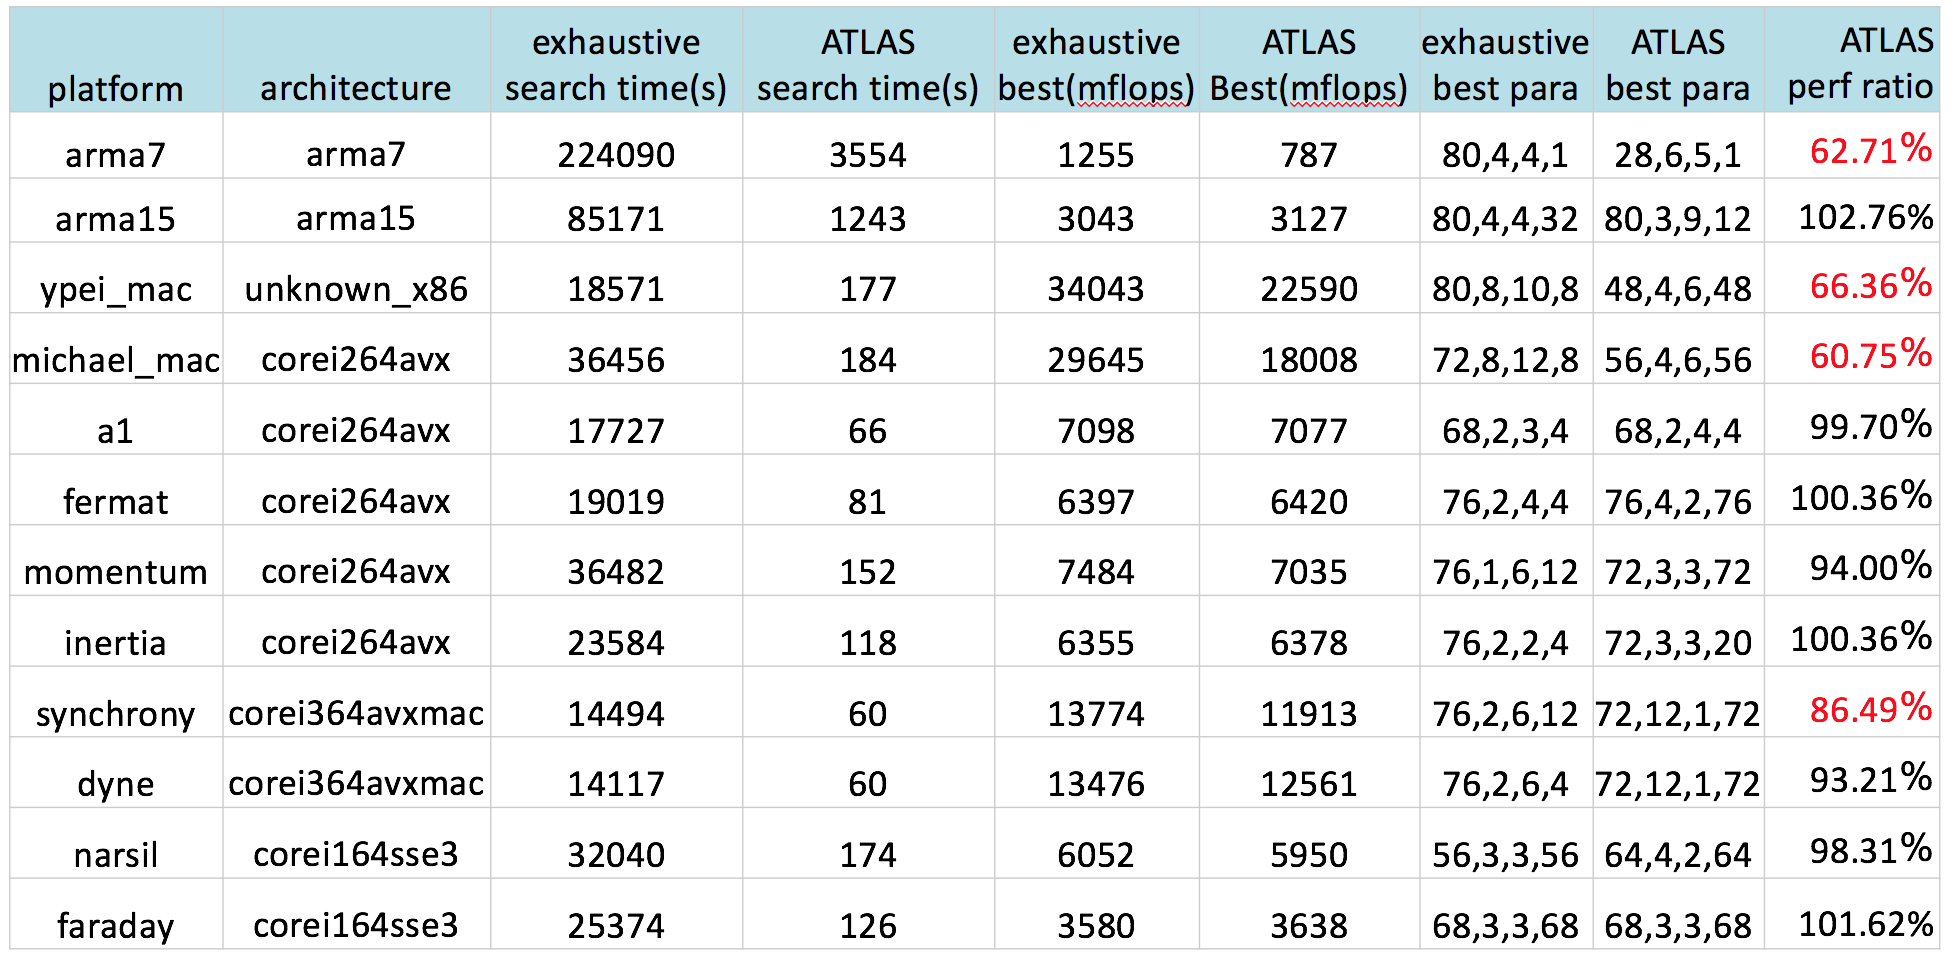
\includegraphics[width=0.9\textwidth]{images/exhaustiveVsorthogonal.png}
    \caption{Searching time comparison between exhaustive search and \atl orthogonal search}
    \label{fig:exhaustiveVsorthogonal}
  \end{figure*}
  In this section, we compare the result of \atl orthogonal search with the best of exhaustive
  search. The search time, generated code performance, and selected parameters are listed in Figure
  \ref{fig:exhaustiveVsorthogonal}.\par
  Except for the two ARM processors, it takes around one to three minutes for ATLAS orthogonal search
  to generate its best code. Considering that we only search for single precision, real number general
  matrix multiplication, we haven't run double precision, complex number or some other benchmarks
  like transpose matrix kernel, matrix vector kernel, big matrix kernel, rank-1 matrix kernel etc, installing
  ATLAS may take hours to finish. The orthogonal search is still too slow to end user.\par
  Column \textit{exhaustive best} and \textit{ATLAS best} list the MFLOPS performance of generated code from
  both search strategy. The ratio of ATLAS over exhaustive is in the last column. On 8 platforms,
  ATLAS is able to generate code with >90\% of best performance. Three platforms has only around 60\% of
  best performance. The two parameter columns list the selected parameters in the order of $(NB, MU, NU, KU)$.\par
  Note for the two MAC platform that, the two middle parameters (MU, NU) are so large that it exceeds
  the register requirement of \[ MU*NU + MU + NU + LS < NR \]. Thus ATLAS orthogonal search is not able
  to find it. Currently we do not have a clear explanation to this. One guess is that, the CORE i7 processors
  have more physical registers than ISA architecture register. The ISA is only able to use or identify 32 registers.
  However due to register renaming, it can make use of more than 32 registers and the extra registers are not visible
  to softwares.\par

  \subsection{GEMM performance model}
  \label{sec:GEMMperf}
  This section discuss whether it is easy to build a model of \gem performance
  given platform information and a knob setting. Intuitively, we evaluate
  whether the \gem performance is predictable. In Fig.\ref{fig:inertia_perf},
  we shows the performance prediction accuracy on platform inertia using a model
  trained by M5 on the other 11 platforms. Each point represent one knob
  setting. This figure shows the comparison between the normalized actual
  performance and the predicted performance. There are two views to evaluate
  this figure. The first view is to see the distance between the points to the
  $y=x$ line. The distance evaluates how accurate the model is.

  Another point of
  view is to focus on the few highest data points, which are the points in the
  red oval in Fig.\ref{fig:inertia_perf}. These points represent the highest
  predicted performance, which will be selected as the candidate knob settings
  in \atl evaluation. The corresponding x axis value is the actual performance
  number for this knob setting. Intuitively, the lefter the point is, the
  better the prediction is, we want high prediction to indicate high actual
  performance. Note that only the knob settings with high performance are
  interested, so the prediction accuracy for low points doesn't matter much in
  this case as soon as high prediction point are left enough.

  Inertia is doing well in both of the views, while platforms like arma7 is not
  because it's really hard to use data collected from 10 Intel processors and 1
  ARM processor to predict another ARM processor's performance, as shown in
  Fig.\ref{fig:arm_perf}. The predicted knobs only yields around 40\% of the
  actual best performance.
  The overall performance prediction, shown in
  Fig.\ref{fig:overall_perf}, is generated by randomly selecting 80\% and 20 \%
  of the data set formed by 12 platforms as training data and testing data
  respectively. It shows the overall difficulty of modeling \gem performance
  is not hard.

  \begin{figure}[bhp]
    \centering
    \begin{subfigure}[b]{1.0\linewidth}
      \centering
      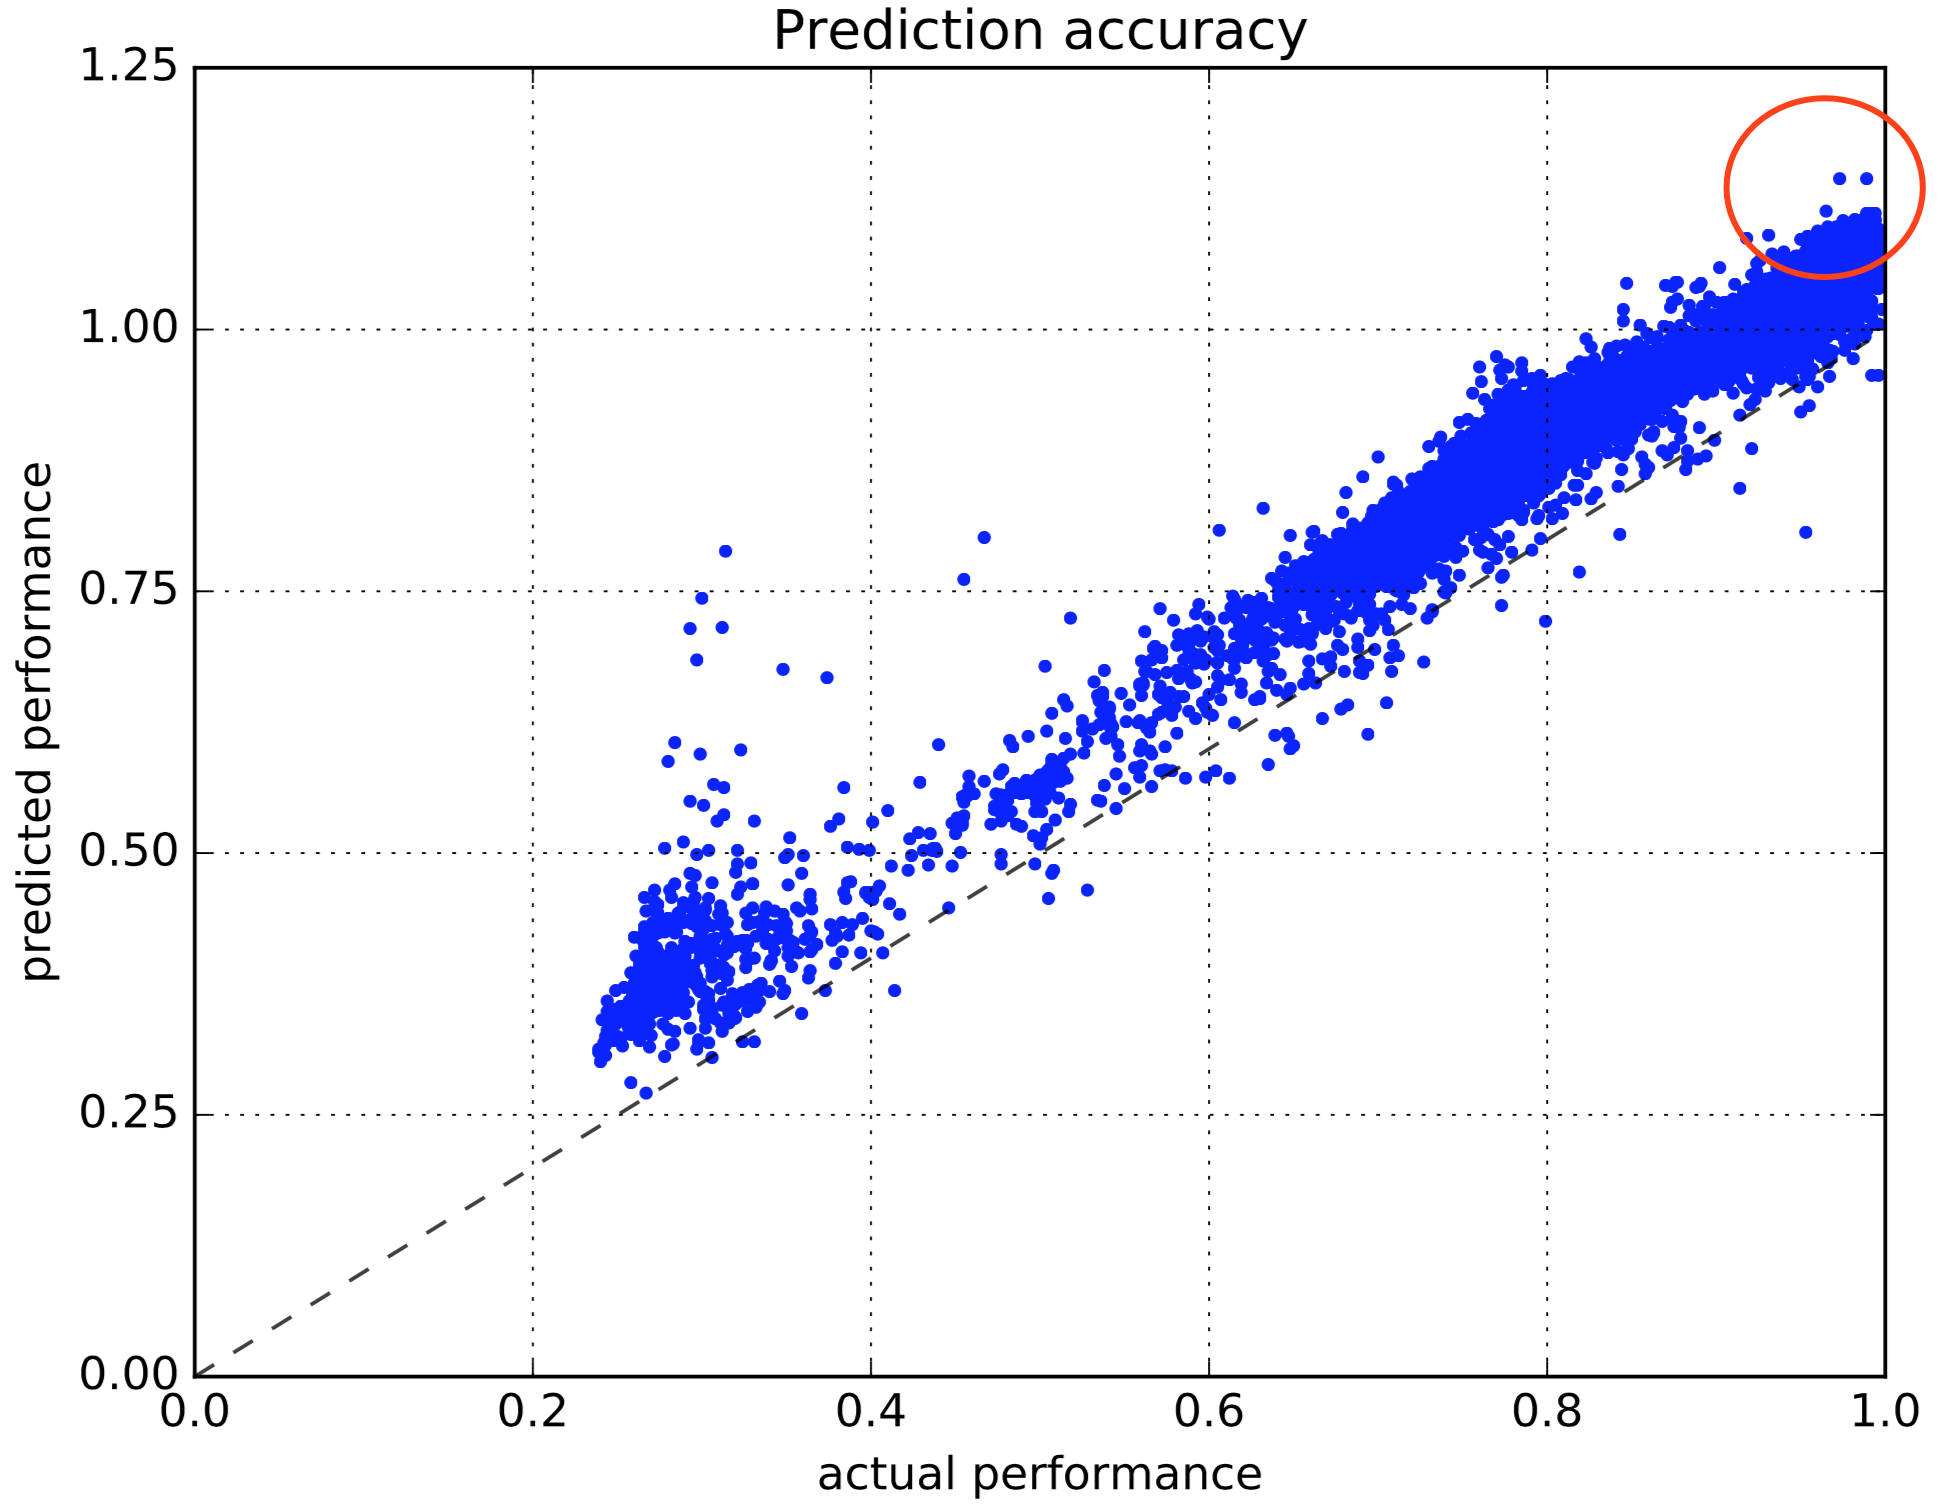
\includegraphics[width=0.8\textwidth]{images/inertia_perf.png}
      \caption{Inertia performance prediction}
      \label{fig:inertia_perf}
    \end{subfigure}
    \begin{subfigure}[b]{1.0\linewidth}
      \centering
      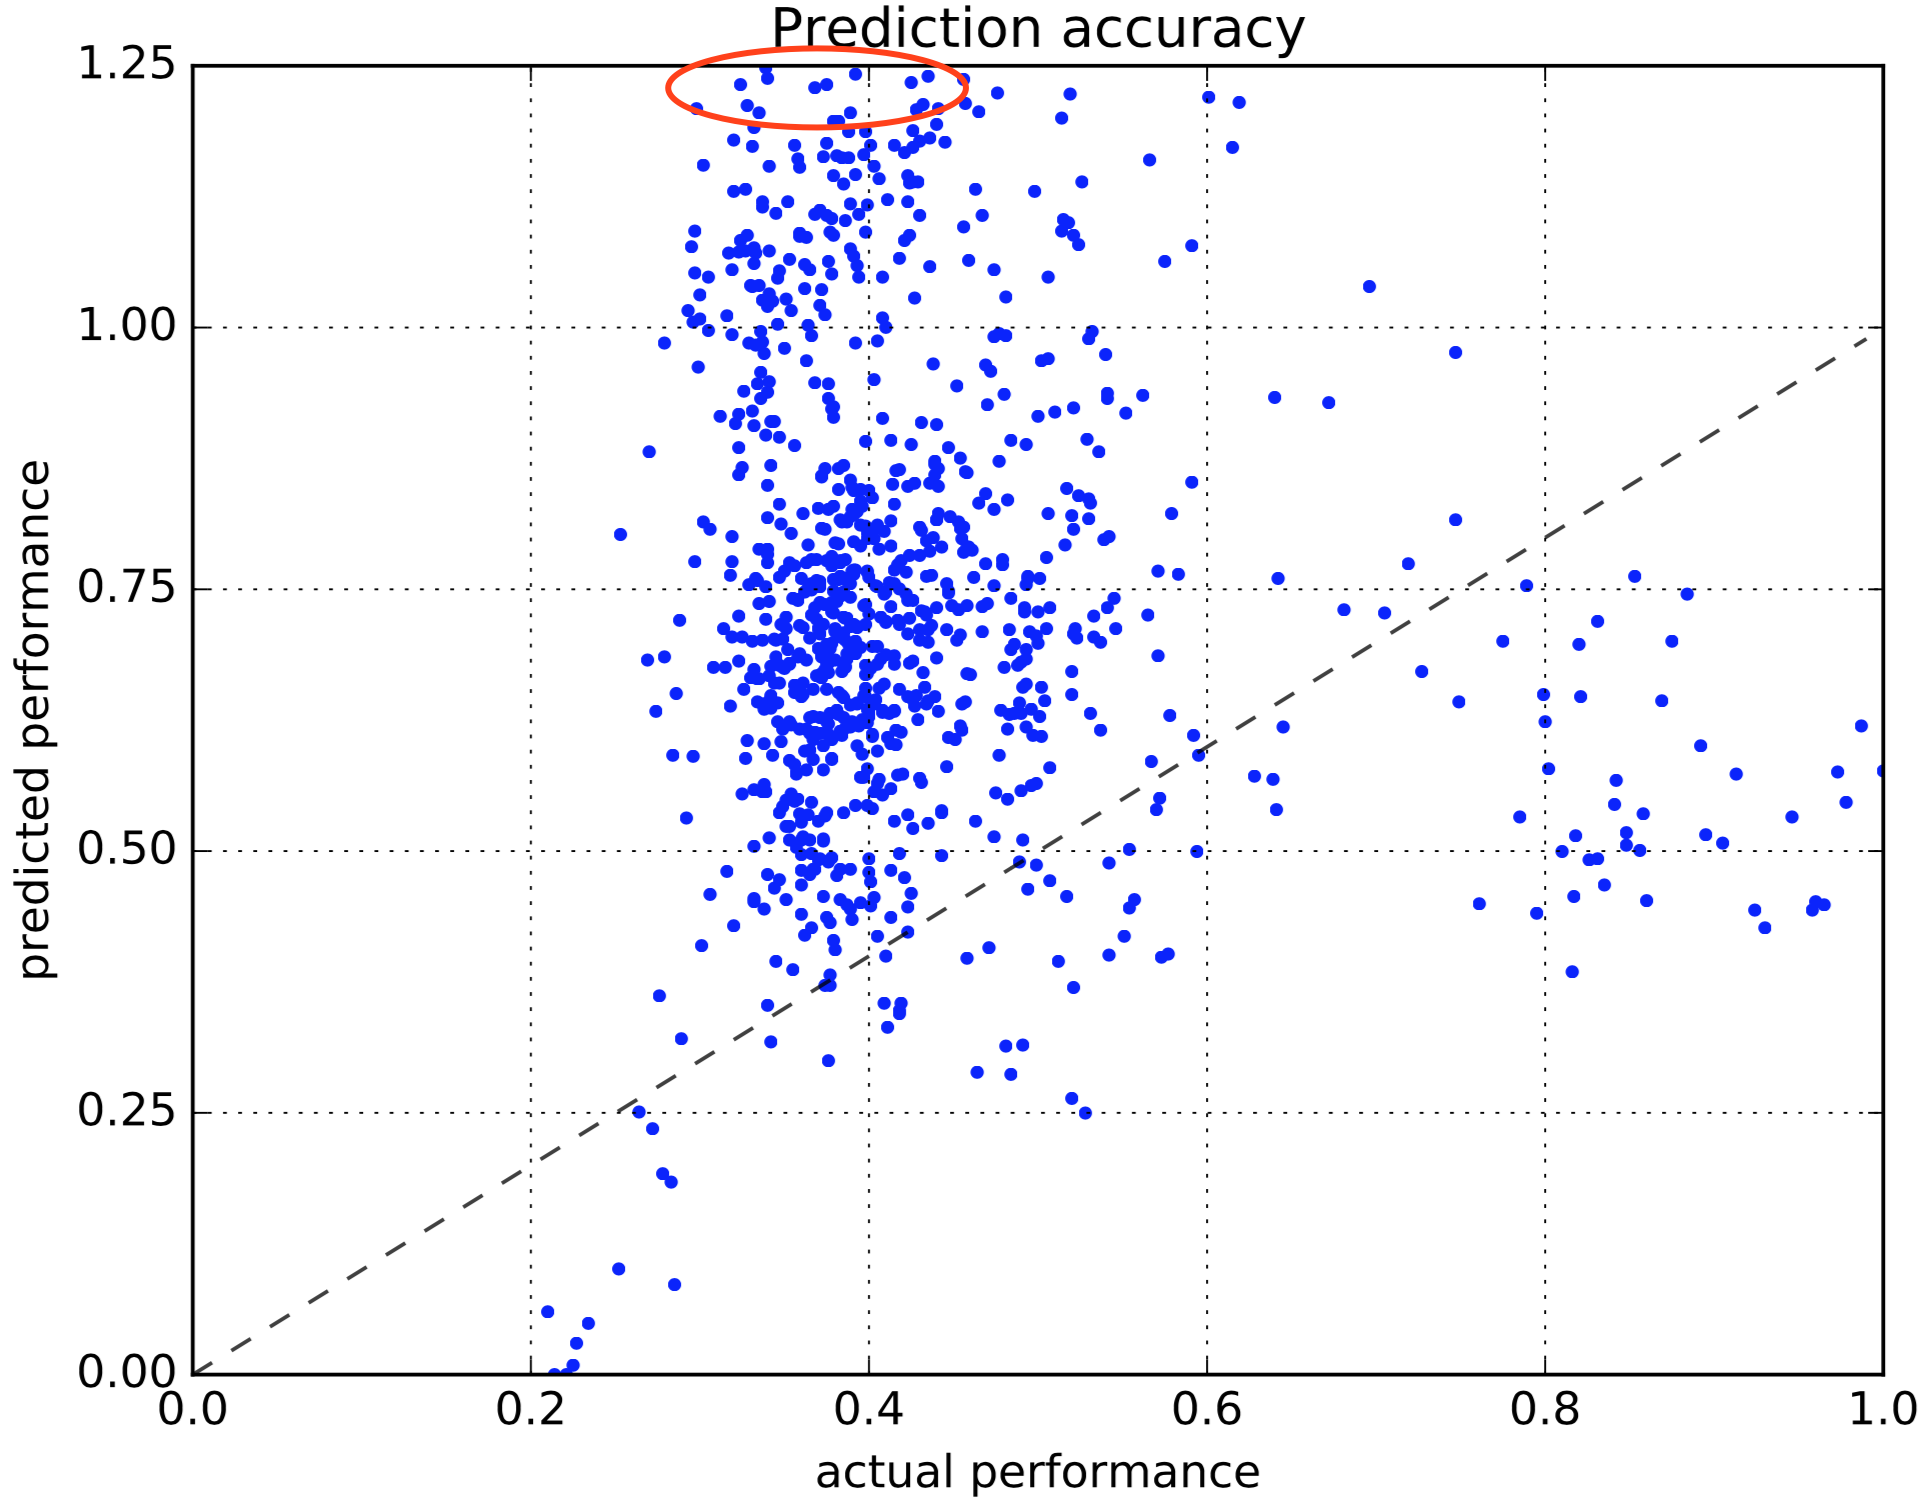
\includegraphics[width=0.8\textwidth]{images/arm_perf.png}
      \caption{Arma7 performance prediction}
      \label{fig:arm_perf}
    \end{subfigure}
    \begin{subfigure}[b]{1.0\linewidth}
      \centering
      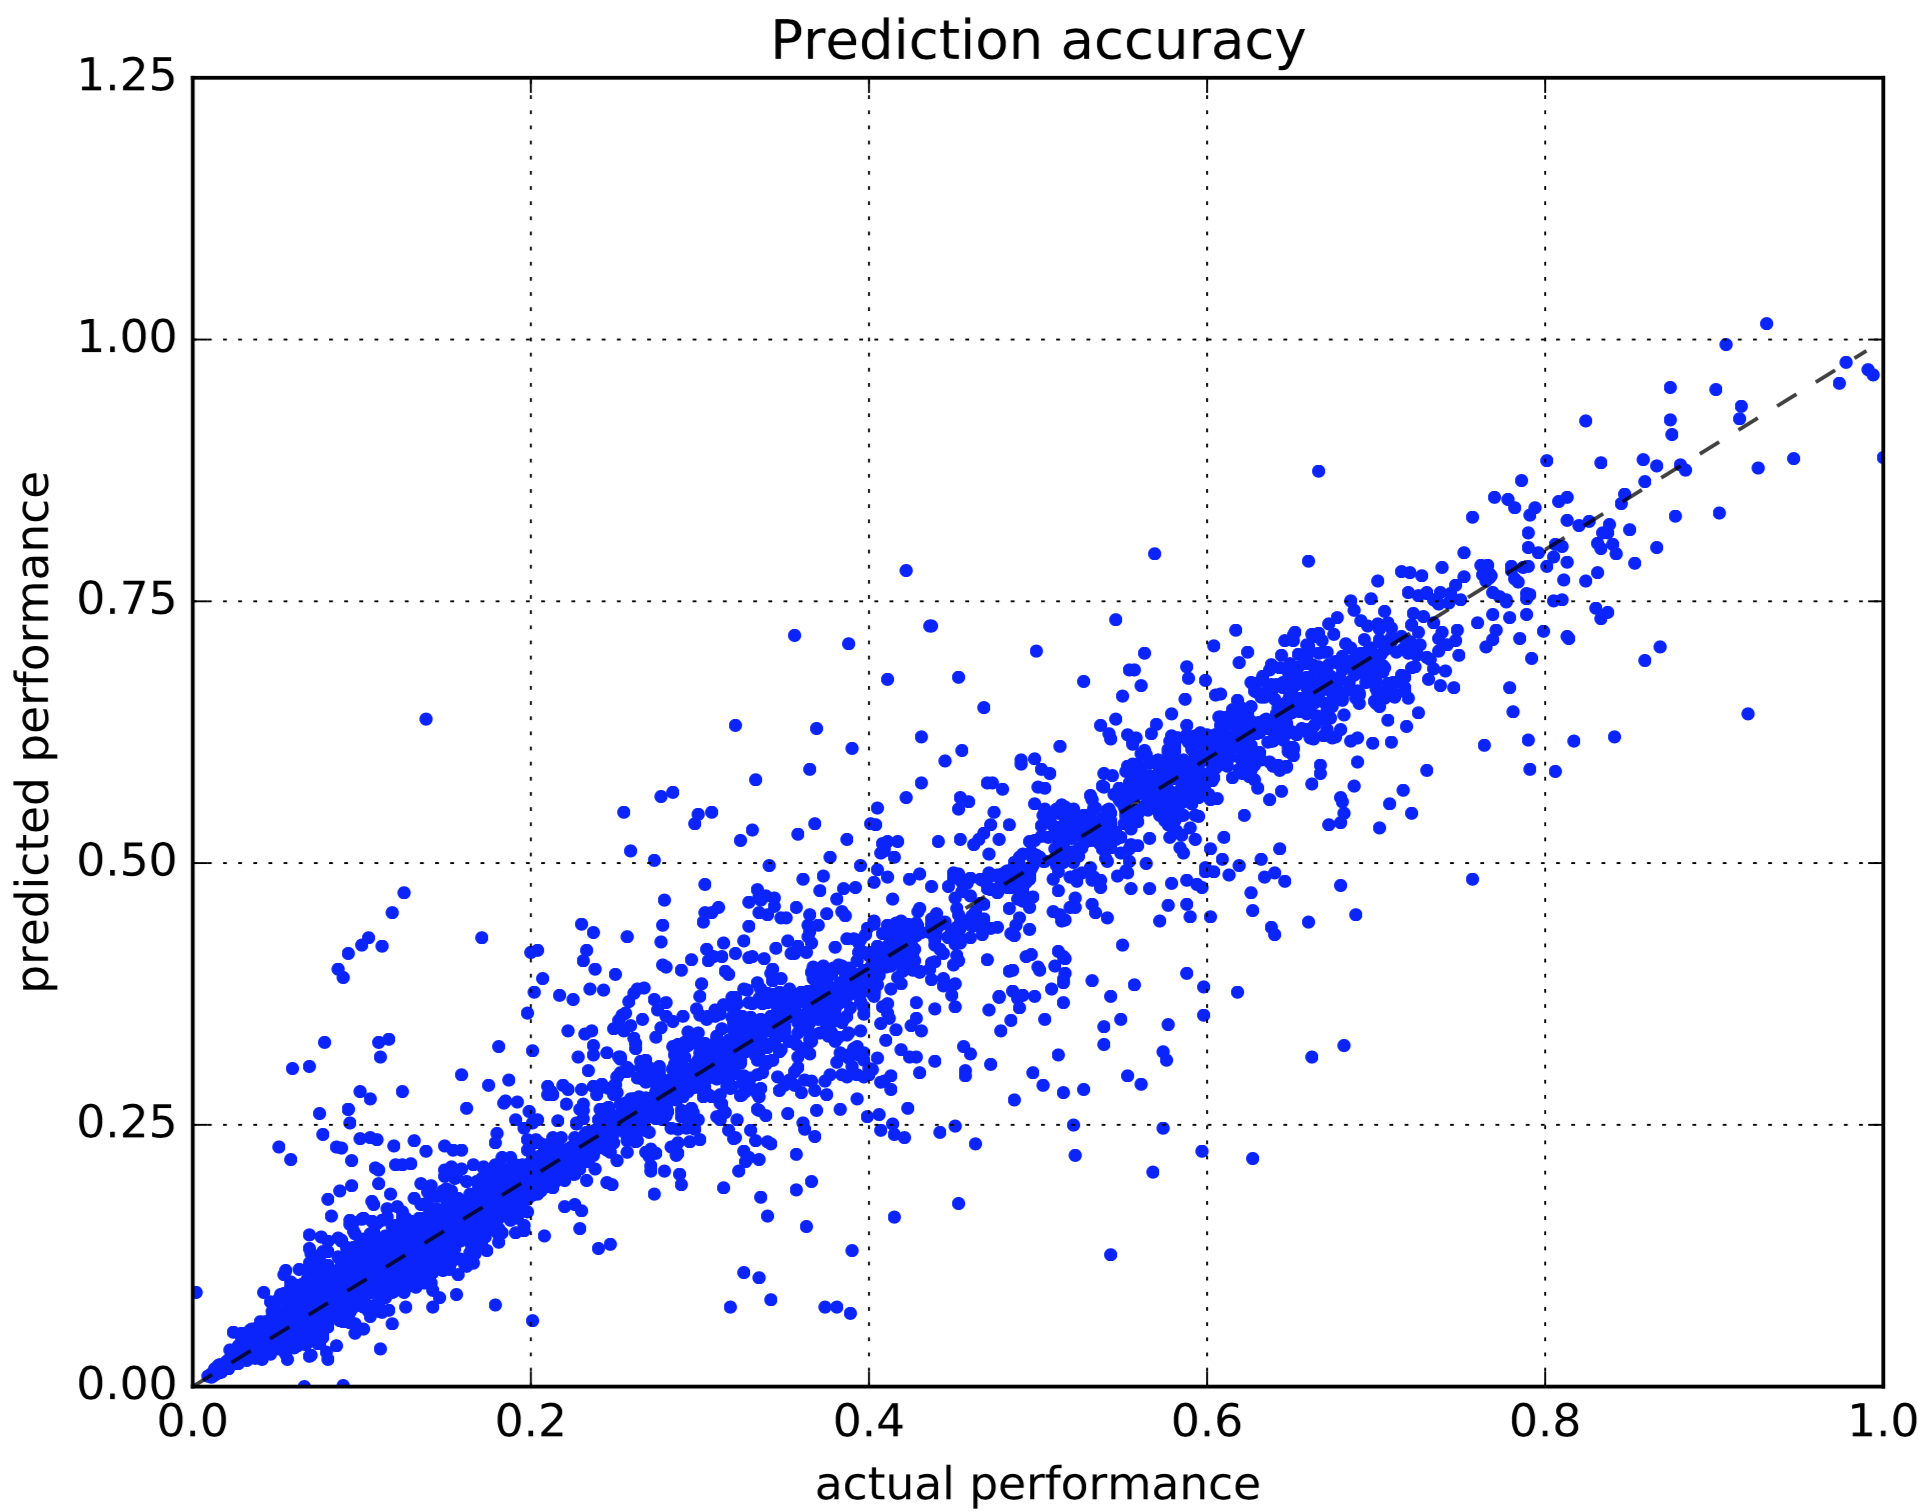
\includegraphics[width=0.8\textwidth]{images/overall_model.png}
      \caption{Overall performance prediction}
      \label{fig:overall_perf}
    \end{subfigure}
    \caption{Performance prediction accuacy overview}
  \end{figure}



  \subsection{Capri-based ATLAS searching time}
  \label{sec:capri_atlas_searching}
  \begin{figure*}[tbhp]
    \centering
    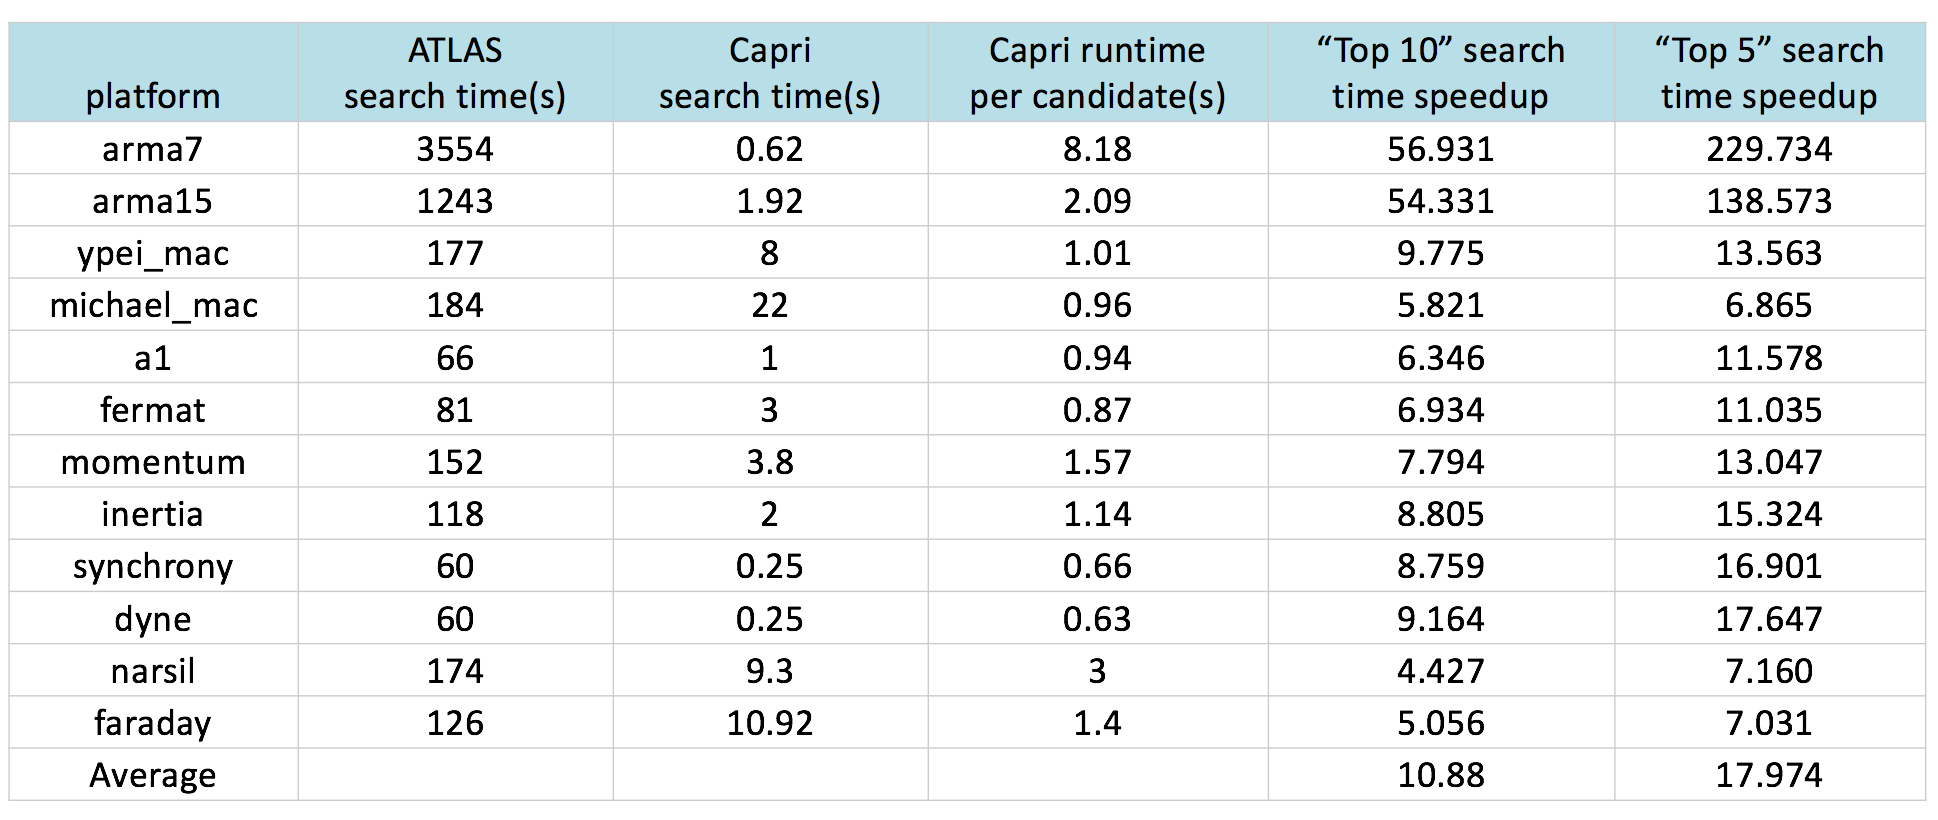
\includegraphics[width=0.9\textwidth]{images/timespeedup.png}
    \caption{Capri-based ATLAS searching time speedup}
    \label{fig:search_time}
  \end{figure*}

  In this section we compare one of our evaluation metric: searching time. An overview of the result is listed in
  Figure \ref{fig:search_time}. The \textit{ATLAS search time} column is the same as in Figure \ref{fig:exhaustiveVsorthogonal}.
  \textit{Capri search time} shows the time Capri takes to purely generate top candidates without running them.
  \textit{Capri runtime per candicates} is the average time of each candidate running on the actual platform.
  Therefore, total Capri-based ATLAS search time which is the sum of \textit{Capri search time} and actual platform time of the candidates,
  highly depends on how many candidates that the user wants. The last two columns show the speedup over ATLAS when users pick
  10 or 5 candidates. On average, Capri-based search outperforms ATLAS orthogonal search by \textbf{10.88X} on 10 candidates and \textbf{17.97X} on
  5 candidates. On the two ARM platforms, Capri-based search can even reach more than 200X speedup.


  \subsection{Capri-based ATLAS performance}
  \label{sec:capri_atlas_performance}
  This section evaluates the performance degradation compared to exhaustive
  search since searching time of Capri-based \atl has been significantly
  shortened. For each platform, we use the data of the rest 11 platforms to
  perform the training and build the model. In the testing phase, top 10
  knob setting with the highest predicted preformance are extracted from the
  model. For this 10 points, the point with the highest actual performance is
  selected as the final knob setting for code generation. The gap between the
  actual performance of this final knob setting and the actual best performance
  given by the exhaustive search is the performance degradation of the
  Capri-based \atl. Performance degradation numbers are displayed in
  Fig.\ref{fig:all_perf}, using 3 different machine learning models. The bars
  represent the performance ratio compared to exhaustive search's, the higher
  the better. For most of the Intel based processors, the performance ratio is
  close to 100\% for bagging predictor and randomized trees. The overall
  performance ratio is 84\%, 95\%, 95\% when using M5, bagging and randomized
  trees respectively.

  On the other hand, the original \atl suffers 13\% performance degradation
  compared to exhaustive search. We can have the conclusion that the
  performance of Capri-based \atl is better than the original ATLAS's when
  choosing proper machine model while the searching time is significantly
  reduced.

  \begin{figure*}[tbhp]
    \centering
    \begin{subfigure}[b]{1.0\linewidth}
      \centering
      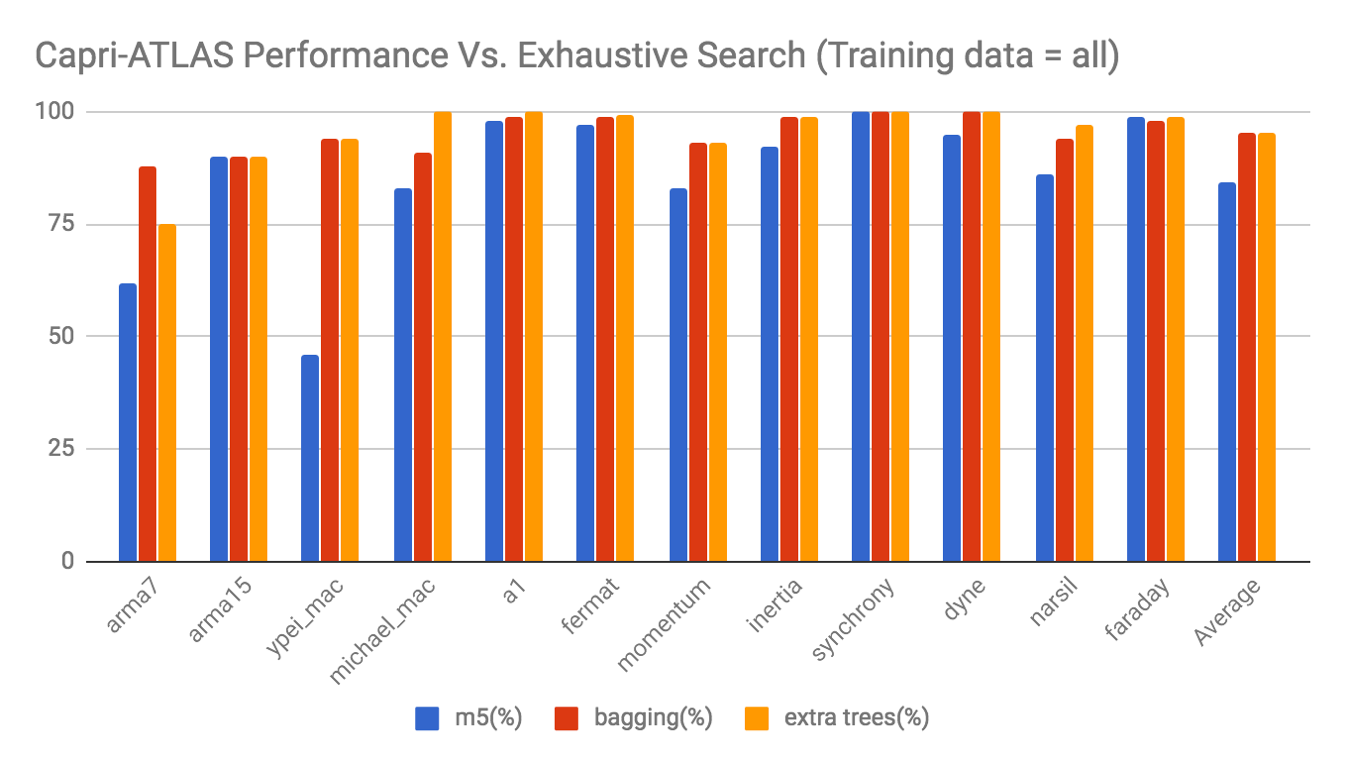
\includegraphics[width=0.85\textwidth]{images/all_perf.png}
      \caption{ }
      \label{fig:all_perf}
    \end{subfigure}
    \begin{subfigure}[b]{1.0\linewidth}
      \centering
      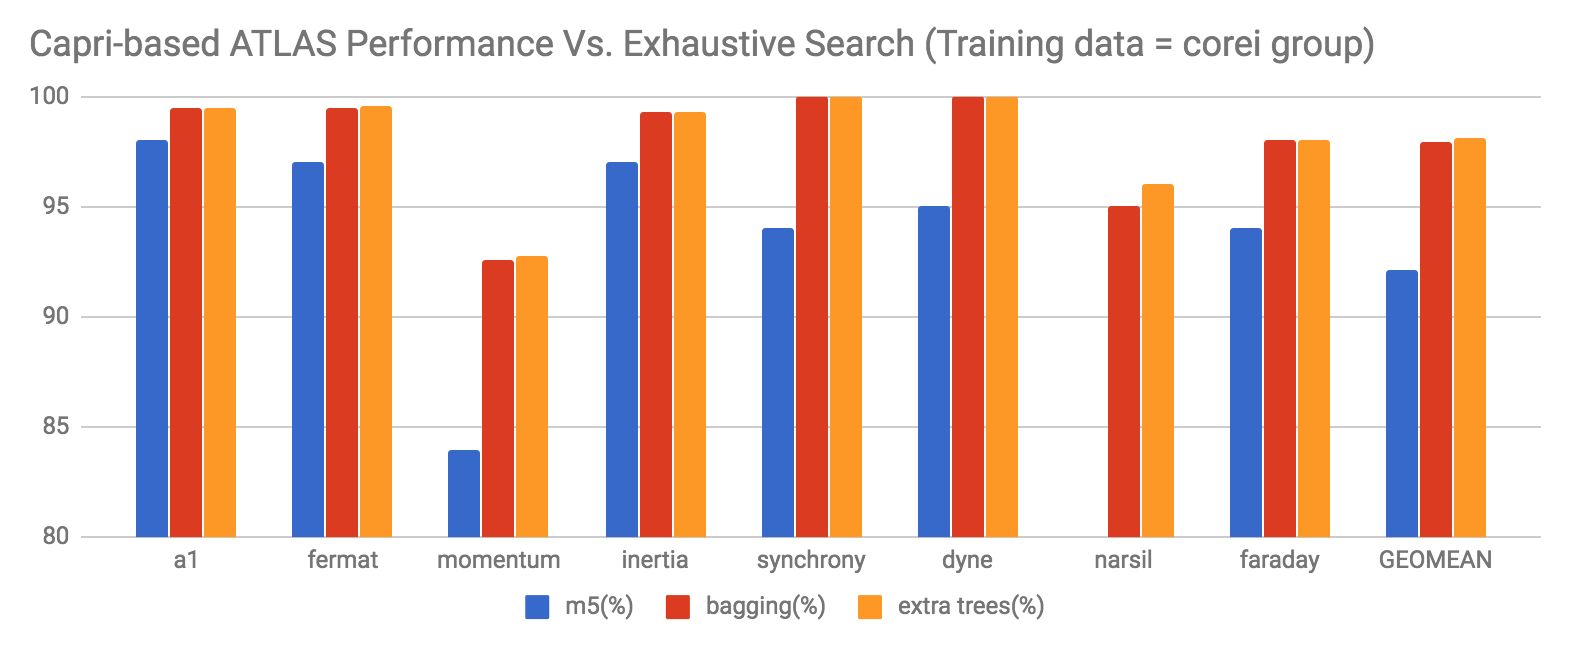
\includegraphics[width=0.85\textwidth]{images/corei_perf.png}
      \caption{ }
      \label{fig:corei_perf}
    \end{subfigure}
    \begin{subfigure}[b]{1.0\linewidth}
      \centering
      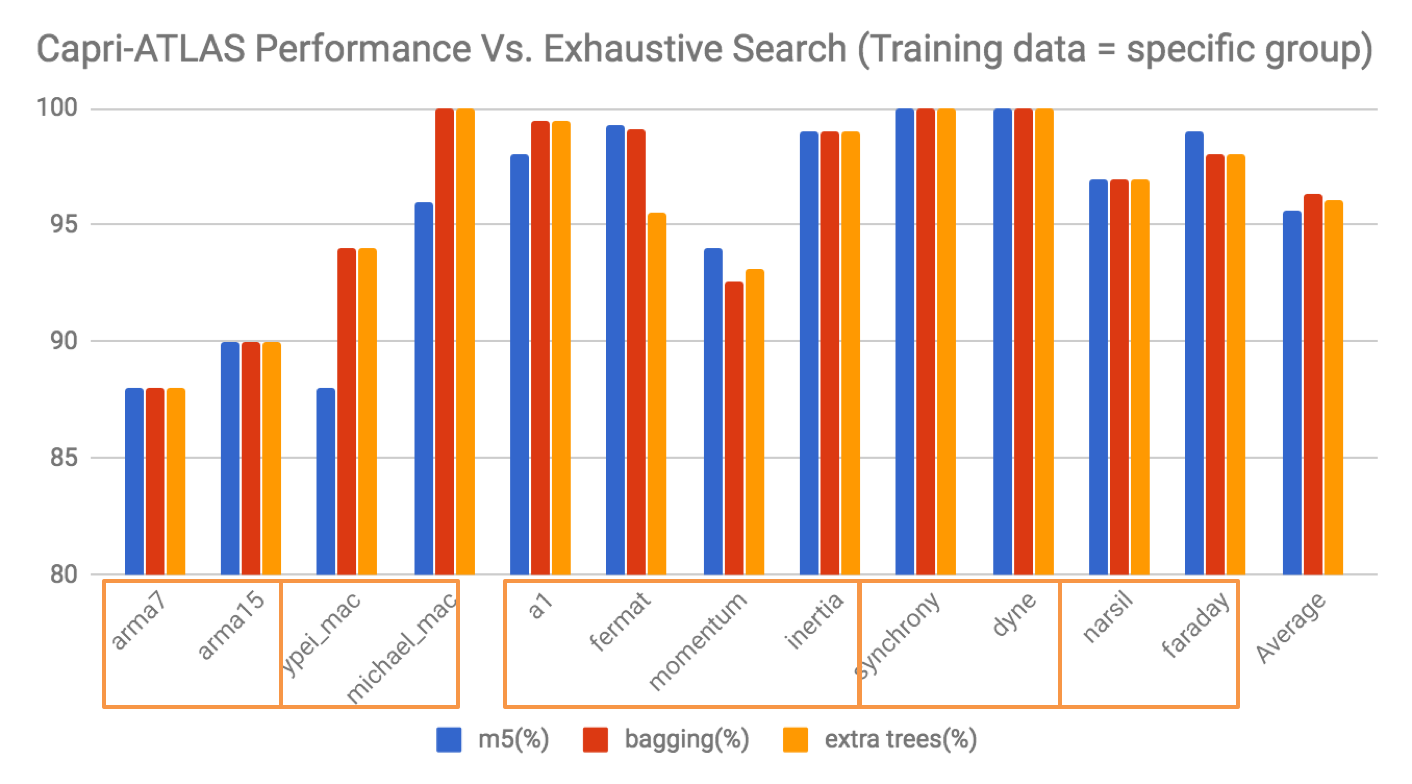
\includegraphics[width=0.85\textwidth]{images/specific_perf.png}
      \caption{ }
      \label{fig:specific_perf}
    \end{subfigure}
  \caption{Capri-based \atl Performance using different training sets}
  \end{figure*}

  \subsection{System sensitivity}
  \label{sec:system_sensitivity}
    The sensitivity of our system should also be evaluated to test its
    practiality. Besides machine learning model selection, two other aspects
    are considered: the influence of training set choice and ``top M''
    constraint.

    \subsubsection{Training set choice}
    \label{sec:training_set}
    \begin{figure*}[tbhp]
      \centering
      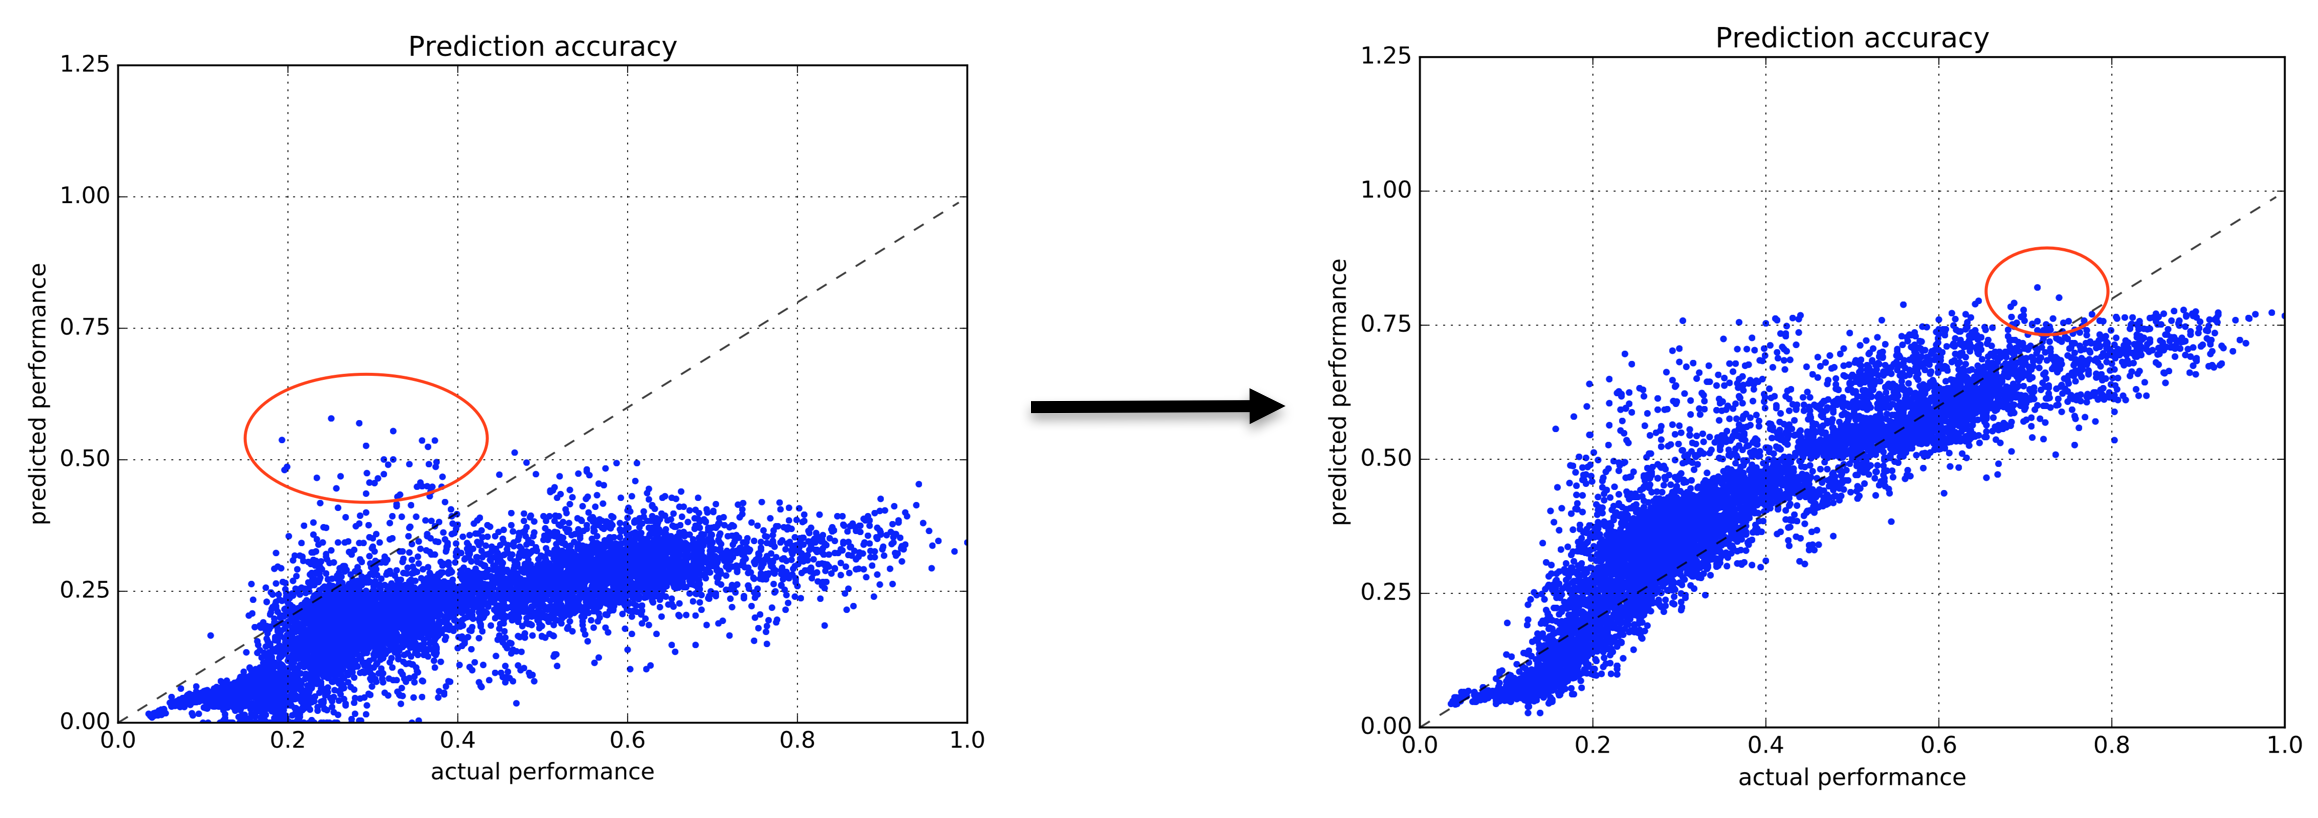
\includegraphics[width=0.9\textwidth]{images/ypei_perf_change.png}
      \caption{Performance improves when a better training set is selected}
      \label{fig:ypei_perf_change}
    \end{figure*}
    The choice of the training set affects the performance of Capri-based \atl
    a lot. Two more sets of experiments are conducted given some prior
    knowledge. For example, if we know that the target platform's architecture
    starts with ``corei'', we can just form the training set with all the
    platforms with the same architecture prefix. Compared to the training set
    that contains everything, this one has less noise. The performance numbers
    of ``corei'' group is given in Fig.\ref{fig:corei_perf}. In addition, we
    also tried more specific training groups whose architectures are the same or
    the compiler settings are the same. The specific groups choice and
    performance number is included in Fig.\ref{fig:specific_perf}. The overall
    performance ratio is 95\%, 96\%, 96\% respectively for specific group cases,
    which has 9\%, 1\%, 1\% performance ratio improvements.

    Note that in Fig.\ref{fig:all_perf} and \ref{fig:specific_perf}, the last
    column shows the geomean only for the 8 ``corei'' platforms (for fair
    comparison with Fig.\ref{fig:corei_perf}). For bagging and randomized
    trees, the performance doesn't have much difference. However, there is a
    performance boost in Fig.\ref{fig:specific_perf} because more suitable
    training set is selected. There is no performance ratio improvements in
    ``corei'' group case is because the ``all'' case has already captured
    the same characteristics as ``corei'' group's.

    To be more intuitive, we show Fig.\ref{fig:ypei_perf_change} to demonstrate
    the difference of choosing different training set. The left one is from
    ``all'' group and the right one is from ``specific'' group using clang as
    the grouping rule.

    \subsubsection{Top M constraint}
    \label{sec:top_m}
    The sensitivity test on the top M constraint is also conducted. In all the
    explanation above, we use top 10 as example. The result for top 5 is
    also collected to evaluate the performance ratio and searching speedup.
    As a result, the top 5 constraint has 80\%, 93\% and 94\% performance ratio,
    which suffers 4\%, 2\% and 1\% ratio decrease. In terms of searching time,
    Capri-based \atl enjoys a overall 17X speedup which is incredible. Note
    that top 5 constraint still performs better than original \atl in both
    performance ratio and searching time. 
